\section{Widgets}
Widgets are the central primitive of the Mosaico ecosystem. They can be thought of as small applications that users can search for, install, and run locally on their matrix through the app store. The Mosaico platform allows anyone to contribute by developing widgets via the developer portal, requiring only a basic knowledge of Python.

\subsection{Widget Types}
Mosaico widgets are categorized into three distinct types:
\label{widget-types}
\begin{figure}[h]
    \centering
    \begin{minipage}[b]{0.32\textwidth}
        \centering
        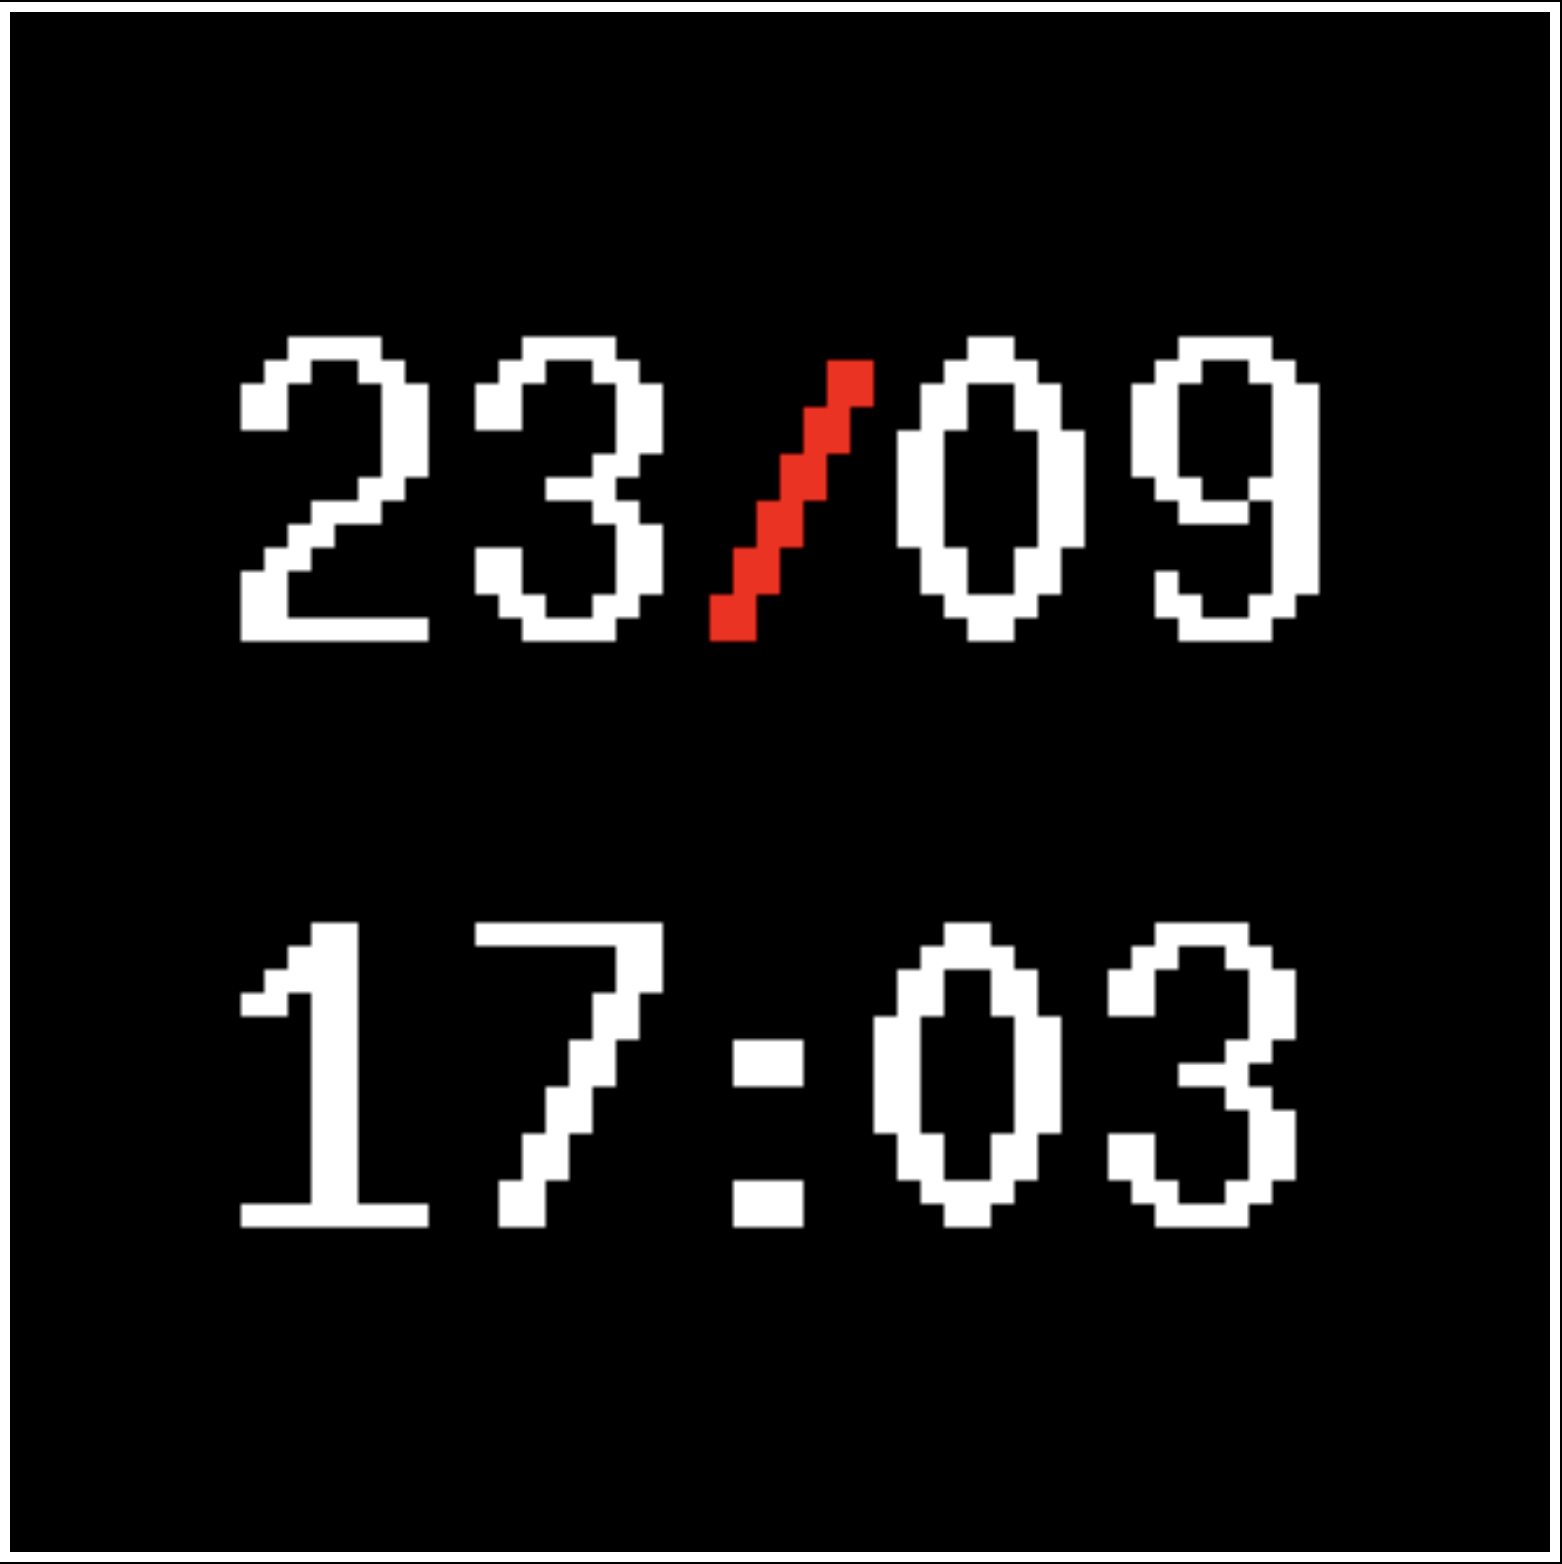
\includegraphics[width=\textwidth]{tesi/img/stylized_widgets/datetime.png}
        \caption*{\textbf{Static Widgets}\newline These can be displayed on the matrix immediately upon installation.}
    \end{minipage}
    \begin{minipage}[b]{0.32\textwidth}
        \centering
        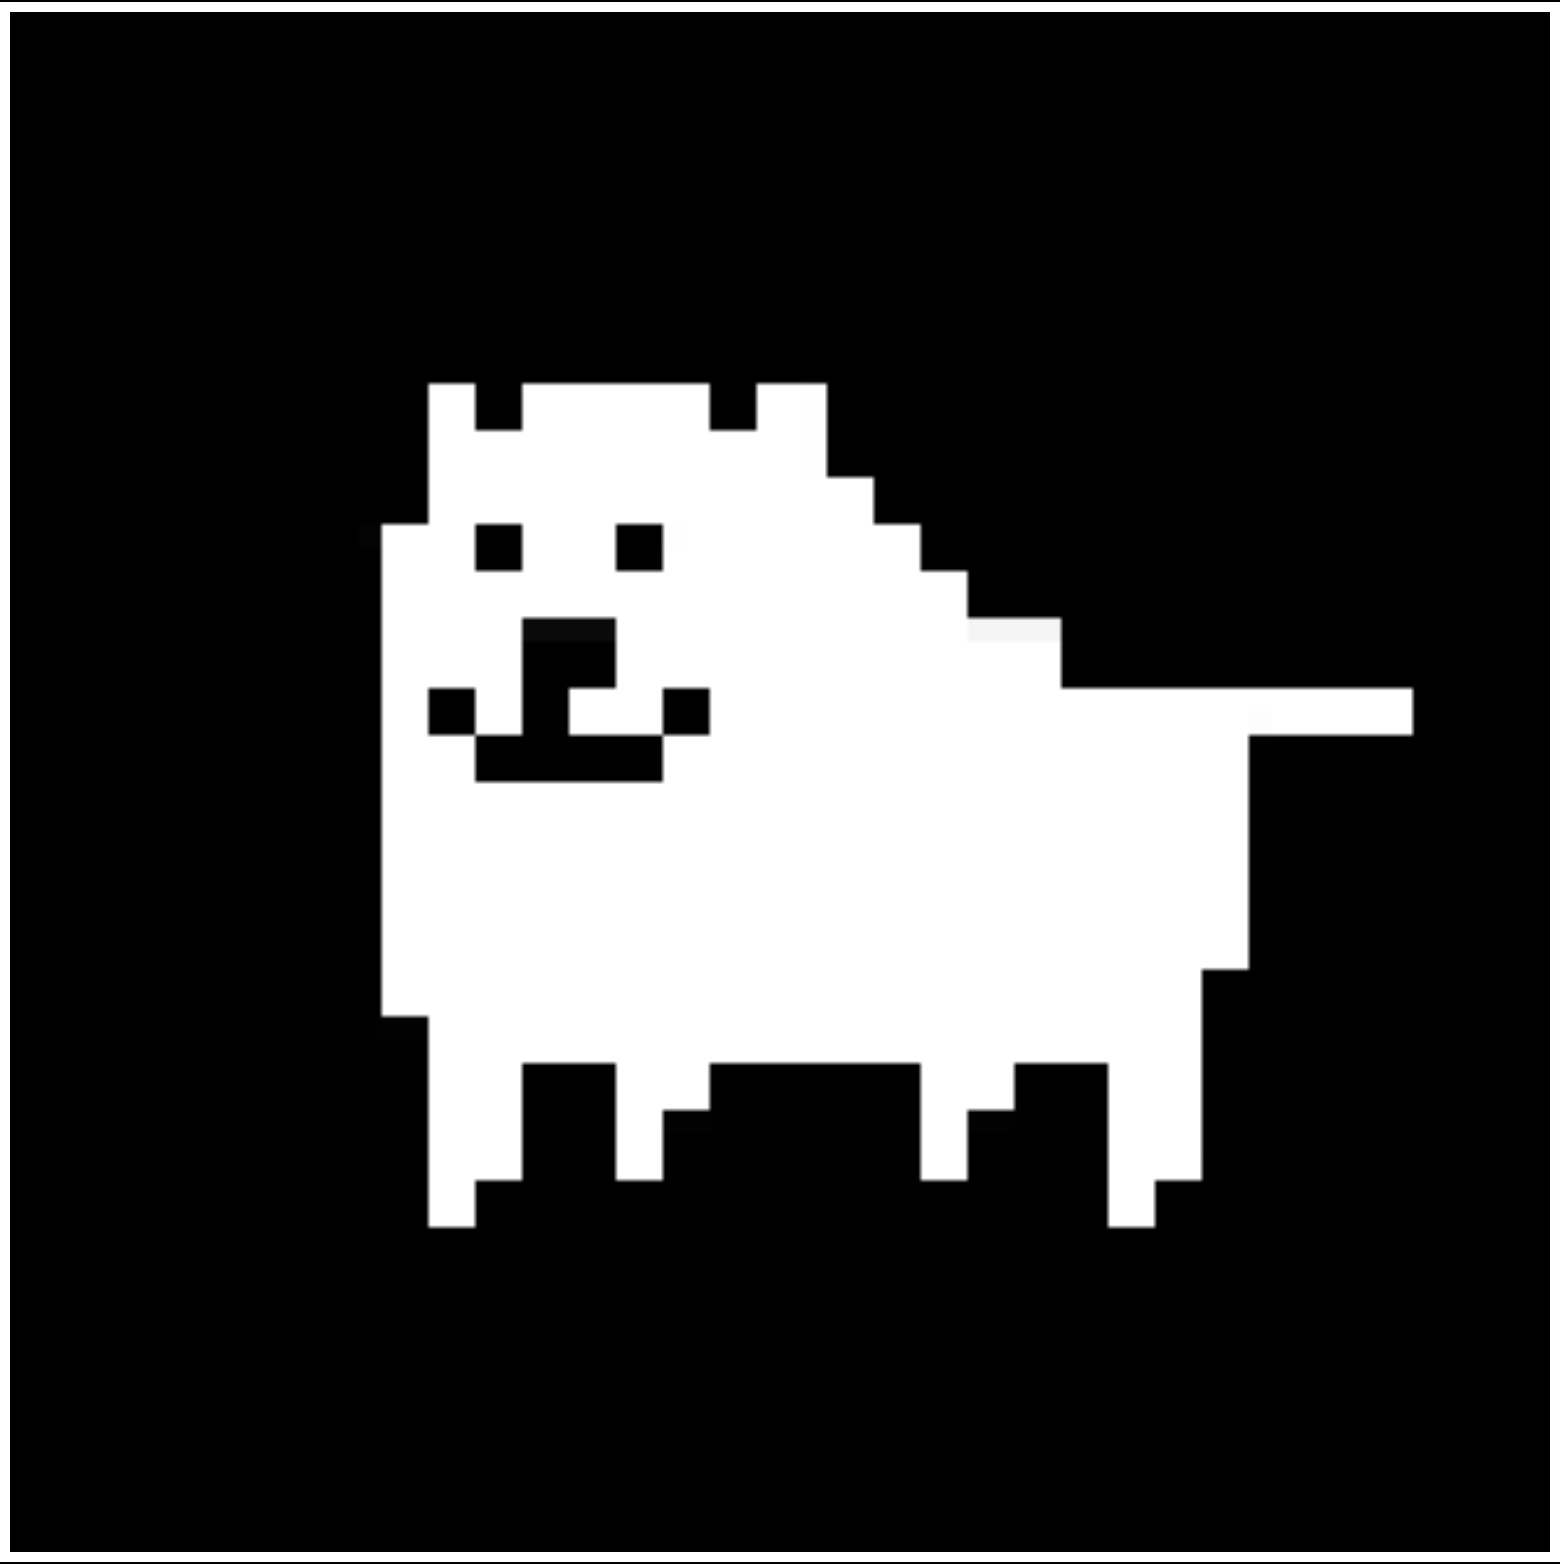
\includegraphics[width=\textwidth]{tesi/img/stylized_widgets/image.png}
        \caption*{\textbf{Configurable Widgets}\newline These require additional configuration before they can be displayed.} 
    \end{minipage}
    \begin{minipage}[b]{0.32\textwidth}
        \centering
        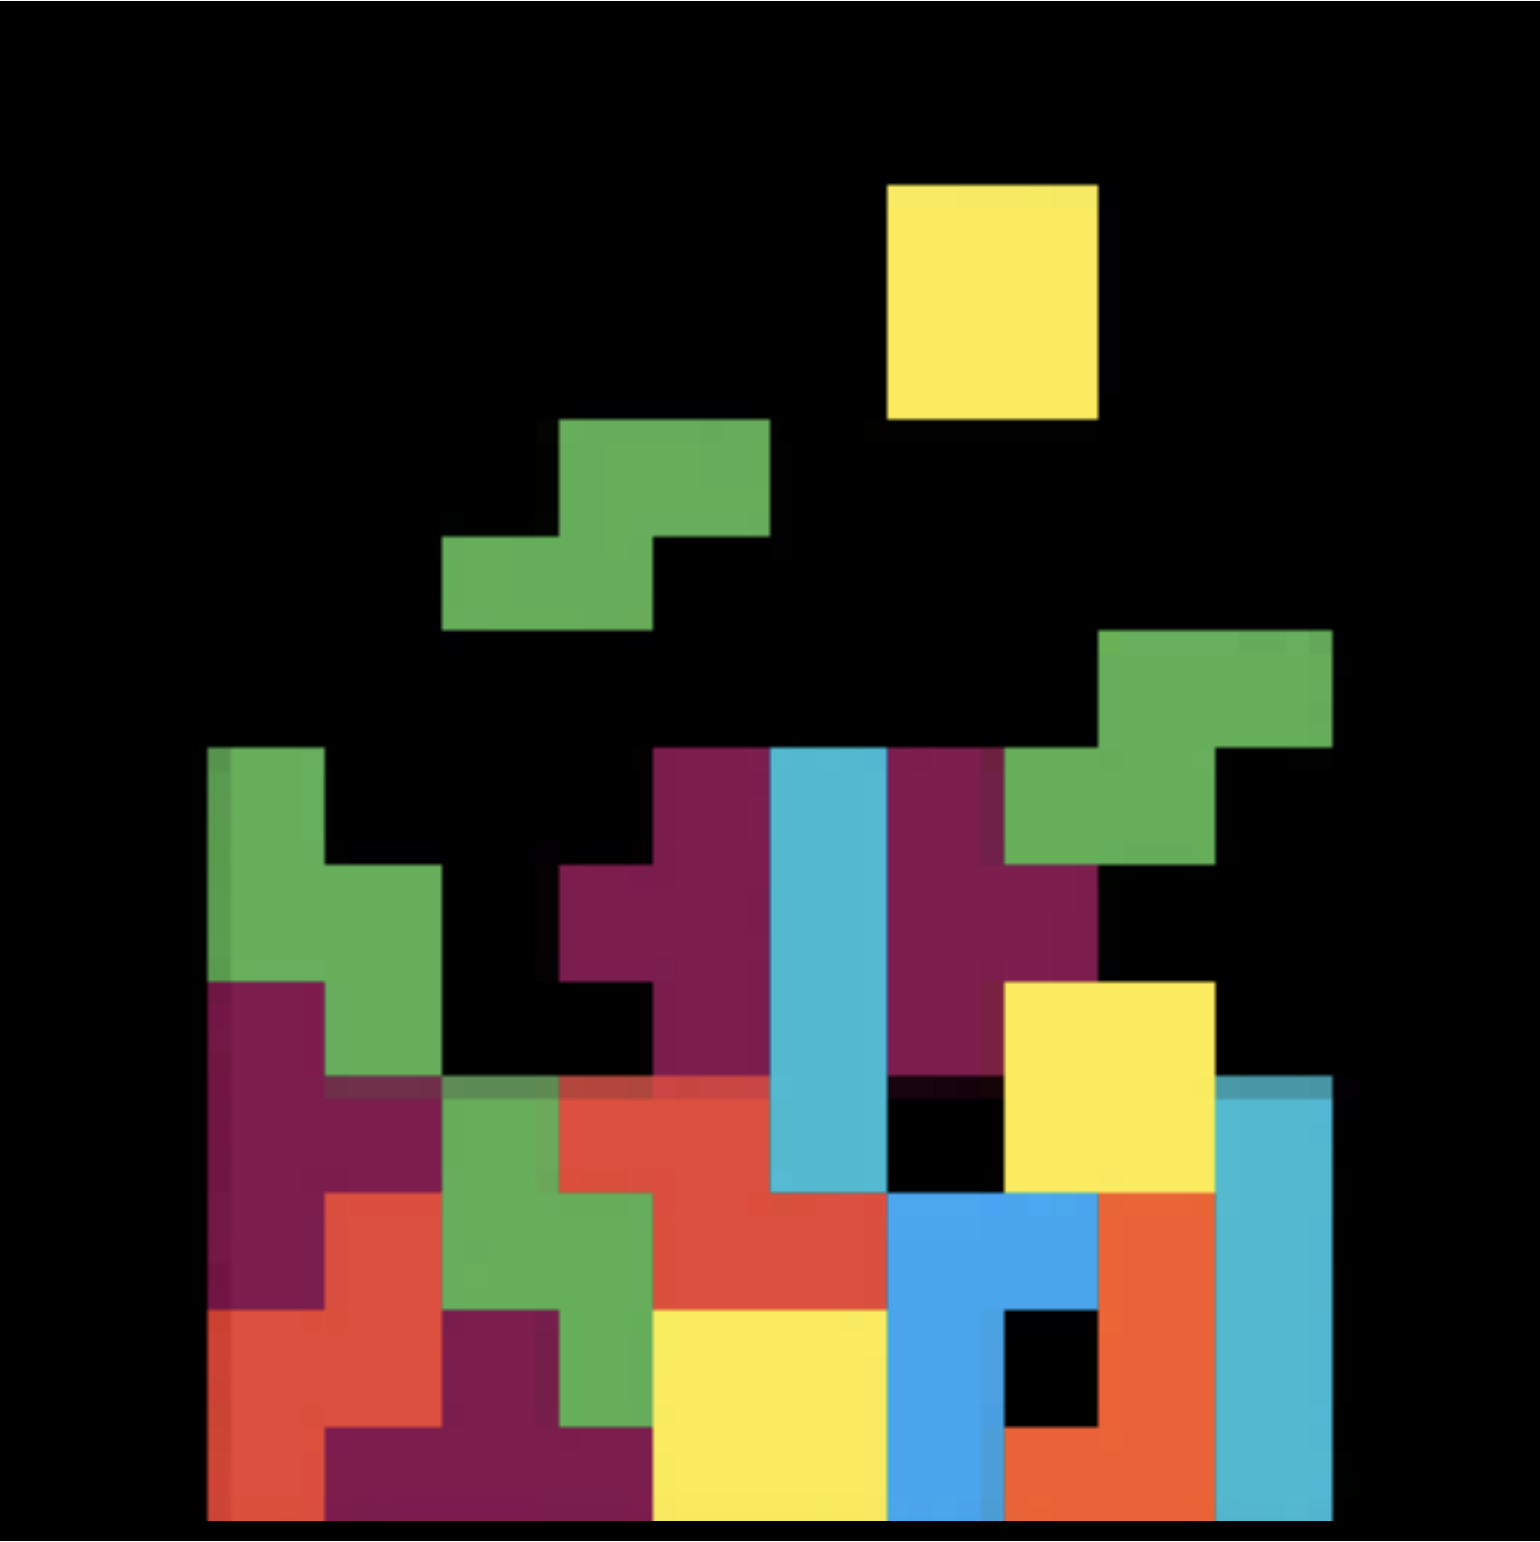
\includegraphics[width=\textwidth]{tesi/img/stylized_widgets/tetris.png}
        \caption*{\textbf{Dynamic Widgets}\newline These require real-time user interaction while they are being displayed.}
    \end{minipage}
\end{figure}

\subsection{Anatomy of a Widget}
We stated what the widgets are and how they play a central role inside the Mosaico ecosystem but how are they actually made?
At their core, Mosaico widgets are projects comprised of three primary components:

\begin{enumerate}
    \item \textbf{Widget Script}: This is the core of the widget, written in Python, and is responsible for rendering visuals on the matrix.

\begin{minted}{python}
# Simple example of a widget that displays "Hello World"
# It retrieves its configuration from the config form
from mosaico import widget, config

# Create text
text = widget.createText()
text.setText(config["text"])
text.setHexColor(config["color"])
text.setFont(config["font"])
text.moveTo(2,30)

# No need to update each frame
def loop():
    pass
\end{minted}

    \item \textbf{Configuration Form}: A JSON file that defines a form to be presented in the client app, collecting input from the user if the widget requires configuration.

\begin{minted}{json}
{
  "form": {
    "title": "Text",
    "description": "Write custom text on the matrix.",
    "fields": [
      {
        "text": {
          "type": "string",
          "label": "Text",
          "required": true,
          "placeholder": "Enter the text you want to display"
        },
        "color": {
          "type": "color",
          "label": "Color",
          "required": true,
          "placeholder": "Choose the color for the text"
        },
        "font": {
          "type": "font",
          "label": "Font",
          "required": true,
          "placeholder": "Select a font"
        }
      }
    ]
  }
}
\end{minted}
\newpage
    \item \textbf{Metadata}: This is a manifest file written in JSON, containing essential information for both the rendering engine (e.g., frame rate, whether the widget is configurable) and the app store platform (e.g., widget name, description, version).

\begin{minted}{json}
{
  "name": "Text",
  "description": "Displays custom text on the matrix.",
  "widget_version": "1.0",
  "software_version": "1.0",
  "author": "murkrow",
  "fps": 20,
  "configurable": true
}
\end{minted}
\end{enumerate}
